%
%%%%%%%%%%%%%%%%%%%%%%%%%%%%%%%%%%%%%%%%%%%%%%%%%%
% PLANTILLA EJERCICIOS DE HISTORIA DE LA MÚSICA I
% Este es un modelo para redactar los ejercicios
% 
% Pasos para cubrir la plantilla:
% 1) Realizar una copia de este modelo
% 2) Renombrar el archivo:
%		"HM1_Hoja(número).tex"
% 3) El número de Hoja debe ser correlativo
% 
%%%%%%%%%%%%%%%%%%%%%%%%%%%%%%%%%%%%%%%%%%%%%%%%%%
%
% Esta plantilla es para crear ejercicios de esta materia
% Se recomienda crear un archivo por cada tema
% Descomentar según se necesite utilizar un modelo de ejercicio u otro
% Clase de documento:
\documentclass[letterpaper,12pt,notitlepage,spanish]{article}
%
% Archivo externo de configuración
% --------------------------------
% Seleccionar o idioma:
%%%%%%%%%%%%%%%%%%%%%%%%%%%%%%%%%%%%%%%%%%%
%% ---------- MODELO EJERCICIOS ---------- 
%% MATERIA: HISTORIA
%% CURSO: 
%% AÑO ACADÉMICO: 
%% CENTRO: 
%%%%%%%%%%%%%%%%%%%%%%%%%%%%%%%%%%%%%%%%%%%
%% 
%% MODELO PARA REDACTAR EJERCICIOS
%% ===============================
%% 
%% Clase de documento
%% ------------------
%\documentclass[letterpaper,12pt,notitlepage,spanish]{article}
%\documentclass[12pt,a4paper,notitlepage]{article}
%
% Márgenes de documento
% ---------------------
\usepackage[left=2.0cm, right=2.0cm, lines=45, top=2.5cm, bottom=2.0cm]{geometry}
%
% Paquetes necesarios
% -------------------
\usepackage[utf8]{inputenc} % acentos en ES
\usepackage[spanish,activeacute, es-tabla]{babel}
\usepackage{enumerate} % entornos de listas
\usepackage{multicol}  % varias columnas texto
\usepackage{fancyhdr}  % encabezado personalizado
\usepackage{fancybox}  % entornos con cajas
\usepackage{pdfpages}  % páginas pdf
%
\usepackage{lipsum} % generar texto aleatorio "loren ipsum"
\usepackage{environ} 
\usepackage{probsoln} % paquete para soluciones
%\showanswers % para mostrar soluciones
%
%Esto es lo importante. Ponemos la solución al margen.
\NewEnviron{solutionnew}{%
%  \leavevmode\marginpar{\raggedright\footnotesize \textbf{Solución:}\\ \BODY}
%  \textbf{Solución:}\\ \BODY} % sol. con salto de liña
  \small{Solución:} \BODY} % sol. na mesma liña
  {}
\renewenvironment{solution}{\solutionnew}{\endsolutionnew}
%
% FIGURAS EN COLUMNAS:
\newenvironment{Figura}
  {\par\medskip\noindent\minipage{\linewidth}}
  {\endminipage\par\medskip}
% ---
%
% Lineas de encabezado y pié
% --------------------------
\renewcommand{\headrulewidth}{0.5pt}
%\renewcommand{\headrulewidth}{1.0pt}
\renewcommand{\footrulewidth}{0.5pt}
%\renewcommand{\footrulewidth}{1.0pt}
\pagestyle{fancy} % estilo de página
%
% Recuadros y figuras
% -------------------
\newcommand\Loadedframemethod{TikZ}
\usepackage[framemethod=\Loadedframemethod]{mdframed}
\usepackage{tikz}
\usetikzlibrary{calc,through,backgrounds}
\usetikzlibrary{matrix,positioning}
%Desssins geometriques
\usetikzlibrary{arrows}
\usetikzlibrary{shapes.geometric}
\usetikzlibrary{datavisualization}
\usetikzlibrary{automata} % LATEX and plain TEX
\usetikzlibrary{shapes.multipart}
\usetikzlibrary{decorations.pathmorphing} 
\usepackage{pgfplots}
\usepackage{physics}
\usepackage{titletoc}
\usepackage{mathpazo} 
\usepackage{algpseudocode}
\usepackage{algorithmicx} 
\usepackage{bohr} 
\usepackage{xlop} 
\usepackage{bbding} 
%\usepackage{minibox} 
% Texto árabe
\usepackage{mathdesign}
\usepackage{bbding} 
% --
% Tipograía:
% ----------
% Fuente HEURÍSTICA (cómoda de leer)
%\usepackage{heuristica}
% Fuente LIBERTINE (cómoda para apuntes)
\usepackage{libertineRoman}
%\usepackage[proportional]{libertine}
% Fuente ROMANDE (estilo antiguo pero no muy cómoda)
%\usepackage{romande} %
% 
% Encabezado y pié de página (textos)
% -----------------------------------
% Modelo 1:
% ---------
% texto de encabezado izquierda:
%\lhead{\normalfont{Historia de la Música I}}
% texto encabezado centro:
%\chead{\textbf{Ejercicios}}
% texto de encabezado derecha:
%\rhead{\normalfont{curso: 2020/2021}}
% texto pié izquierdo:
%\lfoot{\small{\textit{}}}
% texto pié centrado:
%\cfoot{\textsc{Pág. \thepage }}
% texto pié derecho
%\rfoot{\textit{Pr. $\mathcal{A}$.Kaal}}
% ----------
% Modelo 2:
% ---------
% Encabezado y pié de página (textos)
% -----------------------------------
% texto de encabezado izquierda:
%
%\lhead{
%	\hrule
%	\vspace*{0.20cm}
%	\normalfont{Historia de la Música I}
%	\vspace*{0.10cm}
	%\hrule
%}
% texto encabezado centro:
%\chead{
%	\textbf{Cuestionario de Ejercicios}
%	\vspace*{0.08cm}}
% texto de encabezado derecha:
%\rhead{
%	\normalfont{curso: 2020/2021}
%	\vspace*{0.08cm}}
%
% texto pié izquierdo:
%\lfoot{
	%\begin{center}
		%\vspace*{0.20cm}
		%\hrule
		%\small{
		%Conservatorio Profesional de Música de Viveiro - Avda. da mariña s/n - (27850) Viveiro - Lugo
		%	}
	%\end{center}
%}
% texto pié centrado:
%\cfoot{
	%\vspace*{0.30cm}
	%\hrule
	%\vspace*{0.90cm}
%	\small{- Página \thepage -  }\\
	%\small{Conservatorio Profesional de Música de Viveiro}\\
	%\small{avda. da Mariña s/n}
%}

% ----------
% Modelo 3:
% ---------
% Encabezado y pié de página (textos)
% -----------------------------------
% texto de encabezado izquierda:
%
\lhead{
	\hrule
	\vspace*{0.20cm}
	\normalfont{Historia da Música I}
	\vspace*{0.10cm}
	%\hrule
}
% texto encabezado centro:
\chead{
	\textbf{CADERNO DE EXERCICIOS}
	\vspace*{0.08cm}}
% texto de encabezado derecha:
\rhead{
	\normalfont{curso: 2021/2022}
	\vspace*{0.08cm}}
%
% texto pié izquierdo:
%\lfoot{
	%\begin{center}
		%\vspace*{0.20cm}
		%\hrule
		%\small{
		%Conservatorio Profesional de Música de Viveiro - Avda. da mariña s/n - (27850) Viveiro - Lugo
		%	}
	%\end{center}
%}
% texto pié centrado:
\cfoot{
	%\vspace*{0.30cm}
	%\hrule
	%\vspace*{0.90cm}
	\small{- \thepage -  }\\
	%\small{Conservatorio Profesional de Música de Viveiro}\\
	%\small{avda. da Mariña s/n}
}

% --------
%=====================Algo setup
\algblock{If}{EndIf}
\algcblock[If]{If}{ElsIf}{EndIf}
\algcblock{If}{Else}{EndIf}
\algrenewtext{If}{\textbf{si}}
\algrenewtext{Else}{\textbf{sinon}}
\algrenewtext{EndIf}{\textbf{finsi}}
\algrenewtext{Then}{\textbf{alors}}
\algrenewtext{While}{\textbf{tant que}}
\algrenewtext{EndWhile}{\textbf{fin tant que}}
\algrenewtext{Repeat}{\textbf{r\'ep\'eter}}
\algrenewtext{Until}{\textbf{jusqu'\`a}}
\algcblockdefx[Strange]{If}{Eeee}{Oooo}
[1]{\textbf{Eeee} "#1"}
{\textbf{Wuuuups\dots}}

\algrenewcommand\algorithmicwhile{\textbf{TantQue}}
\algrenewcommand\algorithmicdo{\textbf{Faire}}
\algrenewcommand\algorithmicend{\textbf{Fin}}
\algrenewcommand\algorithmicrequire{\textbf{Variables}}
\algrenewcommand\algorithmicensure{\textbf{Constante}}% replace ensure by constante
\algblock[block]{Begin}{End}
\newcommand\algo[1]{\textbf{algorithme} #1;}
\newcommand\vars{\textbf{variables } }
\newcommand\consts{\textbf{constantes}}
\algrenewtext{Begin}{\textbf{debut}}
\algrenewtext{End}{\textbf{fin}}
%================================
%================================

\setlength{\parskip}{1.25cm}
\setlength{\parindent}{1.25cm}
\tikzstyle{titregris} =
[draw=gray,fill=gray, shading = exersicetitle, %
text=gray, rectangle, rounded corners, right,minimum height=.3cm]
\pgfdeclarehorizontalshading{exersicebackground}{100bp}
{color(0bp)=(green!40); color(100bp)=(black!5)}
\pgfdeclarehorizontalshading{exersicetitle}{100bp}
{color(0bp)=(red!40);color(100bp)=(black!5)}
\newcounter{exercise}
%\renewcommand*\theexercise{exercice \textbf{Ejercicio}~n\arabic{exercise}} % CASTELÁN
\renewcommand*\theexercise{exercice \textbf{Exercicio}~n\arabic{exercise}} % GALEGO
\makeatletter
\def\mdf@@exercisepoints{}%new mdframed key:
\define@key{mdf}{exercisepoints}{%
\def\mdf@@exercisepoints{#1}
}
\mdfdefinestyle{exercisestyle}{%
outerlinewidth=1em,outerlinecolor=white,%
leftmargin=-1em,rightmargin=-1em,%
middlelinewidth=0.5pt,roundcorner=3pt,linecolor=black,
apptotikzsetting={\tikzset{mdfbackground/.append style ={%
shading = exersicebackground}}},
innertopmargin=0.1\baselineskip,
skipabove={\dimexpr0.1\baselineskip+0\topskip\relax},
skipbelow={-0.1em},
needspace=0.5\baselineskip,
frametitlefont=\sffamily\bfseries,
settings={\global\stepcounter{exercise}},
singleextra={%
\node[titregris,xshift=0.5cm] at (P-|O) %
{~\mdf@frametitlefont{\theexercise}~};
\ifdefempty{\mdf@@exercisepoints}%
{}%
{\node[titregris,left,xshift=-1cm] at (P)%
{~\mdf@frametitlefont{\mdf@@exercisepoints points}~};}%
},
firstextra={%
\node[titregris,xshift=1cm] at (P-|O) %
{~\mdf@frametitlefont{\theexercise}~};
\ifdefempty{\mdf@@exercisepoints}%
{}%
{\node[titregris,left,xshift=-1cm] at (P)%
{~\mdf@frametitlefont{\mdf@@exercisepoints points}~};}%
},
}
\makeatother


%%%%%%%%%

%%%%%%%%%%%%%%%
\mdfdefinestyle{theoremstyle}{%
outerlinewidth=0.01em,linecolor=black,middlelinewidth=0.5pt,%
frametitlerule=true,roundcorner=2pt,%
apptotikzsetting={\tikzset{mfframetitlebackground/.append style={%
shade,left color=white, right color=blue!20}}},
frametitlerulecolor=black,innertopmargin=1\baselineskip,%green!60,
innerbottommargin=0.5\baselineskip,
frametitlerulewidth=0.1pt,
innertopmargin=0.7\topskip,skipabove={\dimexpr0.2\baselineskip+0.1\topskip\relax},
frametitleaboveskip=1pt,
frametitlebelowskip=1pt
}
\setlength{\parskip}{0mm}
\setlength{\parindent}{10mm}
%\mdtheorem[style=theoremstyle]{ejercicio}{\textbf{Ejercicio}} % Castelán
\mdtheorem[style=theoremstyle]{ejercicio}{\textbf{Exercicio}} % Galego
%================Liste definition--numList-and alphList=============
\newcounter{alphListCounter}
\newenvironment
{alphList}
{\begin{list}
{\alph{alphListCounter})}
{\usecounter{alphListCounter}
\setlength{\rightmargin}{0cm}
\setlength{\leftmargin}{0.5cm}
\setlength{\itemsep}{0.2cm}
\setlength{\partopsep}{0cm}
\setlength{\parsep}{0cm}}
}
{\end{list}}
\newcounter{numListCounter}
\newenvironment
{numList}
{\begin{list}
{\arabic{numListCounter})}
{\usecounter{numListCounter}
\setlength{\rightmargin}{0cm}
\setlength{\leftmargin}{0.5cm}
\setlength{\itemsep}{0cm}
\setlength{\partopsep}{0cm}
\setlength{\parsep}{0cm}}
}
{\end{list}}
%
%
%% -- Fin del archivo de configuración  --
%% % Galego
%\input{../../Modelos/include/config-HM1ejercicios_ES.tex} % Castelán
% --------------------------------
\usepackage{graphicx}   % Gráficos
\usepackage{hyperref}   % Enlaces
\usepackage{subcaption} % Subfiguras
\usepackage{float}		% Forzar figuras
%
%Ruta absoluta en formato tipo Unix (Linux, OsX)
\graphicspath{{../../../figures}}
%
\setlength{\columnsep}{1cm} % separación entre columnas
\setlength{\columnseprule}{0.75pt}
\begin{document}
%
% DATOS DE HOJA DE EJERCICIOS
% ---------------------------
%
% TÍTULO DE LA HOJA DE EJERCICIOS:
%
\begin{center}
\Large{
2º Trimestre
} \\
\vspace*{0.5cm}
%
% NÚMERO DE HOJA:
%
%\normalsize % Número de hoja:
%(XVII - XVIII)
%\\
\vspace{1.10cm}
	\begin{flushleft}
	Nome e Apelidos: \hrulefill\\
	%\vspace*{0.50cm}
%		\begin{center}
%		\small{Instrucciones para realizar los ejercicios}\\		
%		\end{center}
%	\hrulefill \\
	%\vspace*{0.25cm}
%
%\small{ % INSTRUCCIONES:
%\texttt{Lee con atención y realiza con detenimiento, los siguientes ejercicios teniendo en cuenta lo que se indica en cada uno. \\
%}} % fin instrucciones.
%
	\vspace*{0.25cm}		
 	\end{flushleft}
\end{center}

% ------------------------------------
% ESPACIO PARA REDACTAR OS EXERCICIOS:
% ------------------------------------ 
%
% EXERCICIO 1.- Comentario «Puer natus est»
% -----------------------------------------
%% EXERCICIOS PARA INCLUÍR DENTRO DO CADERNO DE EXERCICIOS %%
%
% EXERCICIO.- COMENTARIO AUDICIÓN PUER NATUS EST NOBIS
%
\section{Un introito gregoriano: «Puer natus est»} \label{sec:Puer-natus}
%
O canto gregoriano é un dos fenómenos musicais máis importantes e identificativos da cultura musical occidental. Naceu coa primitiva igrexa cristiá, con influencias dos cantos de tradición  xudea e greco-romana.
%
Dentro das propostas de análise de audición con partitura de monodia relixiosa medieval, estudamos o «Puer natus est», un introito gregoriano.
%
\subsection*{Análise da audición} 

Para realizar a análise con partitura da audición do introito, seguiremos os pasos que se indican a continuación.
\begin{multicols}{2}
%\begin{enumerate}[1.-]
%PUNTO NÚMERO 1: ESCOITAR A PEZA
%
\subsubsection*{Paso no. 1: análise da partitura} 

No caso de análise dunha audición con partitura prestaremos atención a tódolos elementos formais que observamos na partitura (notación e demáis grafías); son os primeiros elementos a recoñecer a golpe de vista.
Aqueles elementos que son descoñecidos ou non recoñecemos a simple vista, rodearémolos cun círculo para aclarar o seu significado.

\subsubsection*{Paso no. 2: escoita activa} 

Despois da observación e lectura e identificaremos os elementos formais por medio dunha escoita activa da obra.
É moi importante identificar auditivamente todo o que observamos no paso 1.
A escoita activa, axudaranos a determinar a relación música-texto da obra neste caso.

\subsubsection*{Paso no.3: datos da audición} 

Unha vez realizados os pasos 1 e 2 prestaremos atención aos seguintes puntos.
%
    \begin{enumerate}[1.-]
% ANÁLISE DO RITMO DA OBRA:
        \item % RITMO
        \textbf{Ritmo}. Identificamos o ritmo, tendo en conta: pulso, indicacións de compás e outras indicacións dinámicas. 
        Neste caso, estamos ante un ritmo:
        \begin{enumerate}[a)]
            \item mensural 
            \item non mensural 
        \end{enumerate}
% ANÁLISE DA MELODÍA DA OBRA:
        \item %MELODÍA:
        \textbf{Melodía}. Tendo en conta a melodía, determinamos o modo, ámbito e estilo. Prestaremos atención ao perfil melódico e interválica, observando se hai grandes saltos ou mais ben discorre por graos conxuntos.
%        \begin{multicols}{2}
        \begin{enumerate}[a)]
            \item 
            Que intervalos se repiten con maior frecuencia? \dotfill
            \item 
            Cal é o maior intervalo que podemos atopar na peza? \dotfill
            \item
            Podemos afirmar que a melodía se move por graos \dotfill
        \end{enumerate}
%        \end{multicols}
        Vexamos a continuación o Modo, Ámbito e Estilo tendo en conta a melodía:
        \begin{itemize}
% ANÁLISE DO MODO:
            \item % MODO
            \textbf{Modo}.
        \begin{itemize}            
            \item 
            Identifica a clave \dotfill
            \item 
            Cal é a nota \textit{finalis}? \dotfill
            \item
            En que modo básico estamos? \dotfill
            \item
            Cal é a nota máis agura? \dotfill 
            \item
            Cal é a nota máis grave? \dotfill 
            \item
            Que intervalo forma coa final? \dotfill
            \item
            Cal é a nota tenor? \dotfill 
            \item
            En qué modo esta a obra? \dotfill
       \end{itemize}
% ANÁLISE DO ÁMBITO DA OBRA:
            \item % ÁMBITO
            \textbf{Ámbito}. \\
            Fixándonos na nota \textit{finalis} e na máis aguda:
                \begin{itemize}
                    \item
                    Que intervalo forman? \dotfill
                    \item
                    A melodía é de ámbito \dotfill
                \end{itemize}
            \item % ESTILO
            \textbf{Estilo do canto}. \\ Segundo a relación musica-texto, estamos ante un estilo:
                \begin{enumerate}[a)]
                  \item
                  Silábico \dotfill
                  \item
                  Neumático \dotfill
                  \item
                  Melismático \dotfill
                \end{enumerate}
        \end{itemize}
        \item % TIMBRE
        \textbf{Timbre}. \\
        Segundo as características da obra, debemos diferenciar as voces, instrumentos, formacións, agrupacións, ...
            \begin{itemize}
                \item 
                Que timbres recoñeces? \dotfill
                \item
                Polo tanto, trátase de \dotfill
            \end{itemize}
% ANÁLISE DA TEXTURA DA OBRA:
        \item %TEXTURA
        \textbf{Textura}. \\
        Polas características da obra, diferenciamos unha textura melódica \ldots 
            \begin{enumerate}[a)]
                \item 
                De escrita horizontal, monódica
                \item 
                De escrita horizontal, polifónica
            \end{enumerate}
% ANÁLISE DA FORMA DA OBRA
        \item %FORMA:
        \textbf{Forma}. \\
        Determinamos a forma segundo a extensión, textura e estrutura da obra. \\ 
        Convén lembrar aquí a seguinte clasificación:
            \begin{enumerate}[a)]
                \item
                Segundo a extensión:
                \begin{itemize}
                    \item
                    \textbf{Formas maiores}, de diferentes movementos ou grandes dimensións
                    \item
                    \textbf{Formas menores}, un só movemento ou de curta duración
                \end{itemize}
                \item
                Segundo os instrumentos ou voces:
                 \begin{itemize}
                    \item
                    \textbf{Formas vocais}, con intervención da voz humana
                    \item
                    \textbf{Formas instrumentais}, só instrumentos
                \end{itemize}
                \item 
                Segundo a súa estrutura:
                \begin{itemize}
                    \item 
                    \textbf{Formas estruturadas}, ou fixas: aquelas con esquema compositivo determinado
                    \item
                    \textbf{Formas libres}: non respetan aparentemente ningunha estrutura definida
                \end{itemize}
            \end{enumerate}
        \par %Pregunta sobre as Formas
        A que tipo de forma, podemos dicir que se axusta esta obra? 
        \begin{enumerate}[a)]
            \item 
            Forma vocal menor libre
            \item
            Forma vocal menor ternaria
            \item
            Forma vocal maior ternaria
            \item
            Forma instrumental menor ternaria
        \end{enumerate}
        \end{enumerate}
%    \end{multicols}
%
\end{multicols}
%\vspace*{0.25cm}
%
\subsubsection*{Paso no.4: clasificación} 
Unha vez realizada a análise da audición, tendo en conta os datos obtidos no paso 3, clasificaremos a obra tendo en conta sobre todo o ámbito e estilo.
%
% RESUMO DA AUDICIÓN DO EXERCICIO
%
\vspace*{0.25cm}
\begin{ejercicio}[Características principais da audición: «Puer natus est»]

% ESPACIO PARA REDACTAR O COMENTARIO DA AUDICIÓN
%
%\small{Trátase dunha forma vocal menor, de estrutura ternaria; segundo o ámbito e estilo, obedece a un canto antifonal do propio da misa cantado a capella por un coro de voces masculinas; a textura monódica horizontal é propia do canto chá (Gregoriano) en estilo neumático na primeira sección e silábico na segunda, de ámbito reducido escrita no modo \textit{tetrardus auténtico} (VII)     }

        \vspace*{2.78cm}
\end{ejercicio}

% ----------------------
% Partitura de audición:
% ----------------------
%\begin{figure}[h]
%    \centering
%    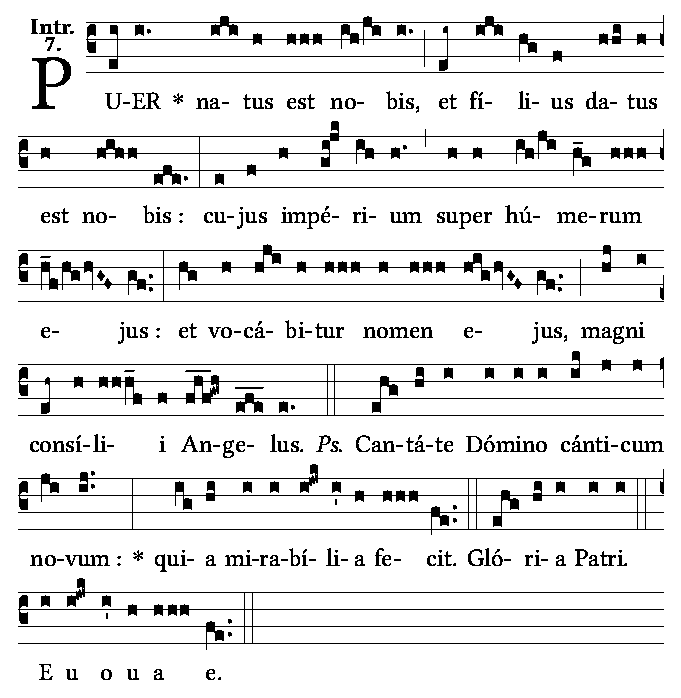
\includegraphics[width=0.75\textwidth]{figures/audicions/Puer-natus.eps}
%    \caption{Partitura do Introito «Puer natus est»}
%    \label{fig:puer-natus}
%\end{figure}
% -----------------------
%
%\newpage
%
% EXERCICIO 2.- Comentario «Viderunt omnes»
% -----------------------------------------
%% EXERCICIOS PARA INCLUÍR DENTRO DO CADERNO DE EXERCICIOS %%
%
% EXERCICIO.- ANÁLISE DA SECUENCIA: Dies irae
%
\section{Análise e comentario do gradual <<Viderunt omnes>>} \label{subsec:Viderunt-omnes}
%
\noindent
Analiza e realiza un breve comentario sobre a obra proposta. Lembra que para realizar a análise con partitura debemos seguir os pasos xa indicados na analise de audición do <<Puer natus est>> (ver o punto \ref{sec:Puer-natus} da páxina \pageref{sec:Puer-natus}). Unha vez obtidos e anotados os datos, realizamos o comentario. \\
Procura información sobre a mesma e realiza unha breve contextualización histórica, social e cultural tendo en conta a época ou período, forma (\ldots). Cita, xunto coa contextualización ao final do comentario, as fontes consultadas.\par
\subsection*{Puntos a indicar}
Debes indicar como mínimo na obra: modo, ámbito, estilo de canto, estrutura formal, clasificación no repertorio e contexto de interpretación


\vspace*{0.15cm}
%
%
% ----------------------
% Partitura de audición:
% ----------------------
\begin{figure}[h]
    \centering
    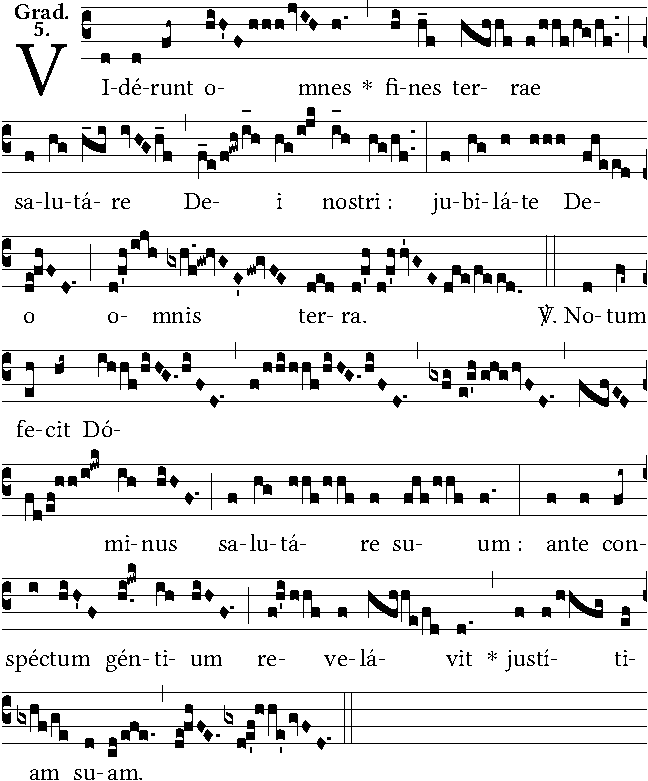
\includegraphics[width=0.70\textwidth]{audicions/viderunt-omnes.pdf}
    \caption{Gradual <<Viderunt omnes>>}
    \label{fig:Viderunt-omnes}
\end{figure}
% -----------------------

% RESUMO DA AUDICIÓN DO EXERCICIO
%
\vspace*{0.5cm}
\begin{ejercicio}[Comentario da audición: <<Viderunt omnes>>]
%\small{
%Redacta un breve comentario da obra. Ten en conta a análise feita:
%}

% ESPACIO PARA REDACTAR O COMENTARIO DA AUDICIÓN
%
%\small{Trátase dunha forma vocal menor, de estrutura ternaria; segundo o ámbito e estilo, obedece a un canto antifonal do propio da misa cantado a capella por un coro de voces masculinas; a textura monódica horizontal é propia do canto chá (Gregoriano) en estilo neumático na primeira sección e silábico na segunda, de ámbito reducido escrita no modo \textit{tetrardus auténtico} (VII)     }

        \vspace*{20.78cm}
\end{ejercicio}


%\newpage
%
% EXERCICIO 3.- Comentario «Dies irae».
% -------------------------------------
%% EXERCICIOS PARA INCLUÍR DENTRO DO CADERNO DE EXERCICIOS %%
%
% EXERCICIO.- ANÁLISE DA SECUENCIA: Dies irae
%
\section{Análise da secuencia <<Dies irae>>} \label{sec:Dies-irae}
%
\noindent
Unha das secuencias máis coñecidas é o <<Dies irae>>, que no século 
{\small XV} empezouse a considerar parte da misa de defuntos, converténdose 
cara finais de século, nun movemento obrigado desta misa.
Para realizar a análise con partitura da audición desta secuencia 
(ilustración \ref{fig:dies-irae}, páxina \pageref{fig:dies-irae}), seguiremos 
os pasos indicados na analise de audición do <<Puer natus est>>  
(apartado \ref{sec:Puer-natus}, páxina \pageref{sec:Puer-natus}); unha vez 
realizada a análise da partitura e escoita activa, completaremos os datos da 
obra.
%
\subsection*{Puntos a indicar} \label{subsec:puntos}
%
\noindent
Analiza e realiza un breve comentario sobre a obra. Procura información sobre a 
mesma e realiza unha breve contextualización histórica, social e cultural tendo 
en conta a época ou período á que pertence, a forma, xénero, estilo, (\ldots). 
Cita, xunto coa contextualización ao final do comentario, as 
fontes consultadas. \\
%
\noindent
Lembra indicar como mínimo na obra: \textbf{modo}, \textbf{ámbito}, 
\textbf{estilo de canto}, \textbf{estrutura formal}, \textbf{clasificación no 
repertorio} e \textbf{contexto de interpretación}
%
\vspace*{0.5cm}
%
% ------------------------
% REALIZACIÓN DO EXERCICIO
% ------------------------

\begin{ejercicio}[Características principais da audición: <<Dies irae>>]

% ESPACIO PARA REDACTAR O COMENTARIO DA AUDICIÓN

%\small{Trátase dunha forma vocal menor, de estrutura ternaria; segundo o ámbito e estilo, obedece a un canto antifonal do propio da misa cantado a capella por un coro de voces masculinas; a textura monódica horizontal é propia do canto chá (Gregoriano) en estilo neumático na primeira sección e silábico na segunda, de ámbito reducido escrita no modo \textit{tetrardus auténtico} (VII)     }

\vspace*{13.5cm}
\end{ejercicio}

%
\newpage
% ----------------------
% Partitura de audición:
% ----------------------
% Forza posición da figura
\begin{figure}[H]
    \centering
    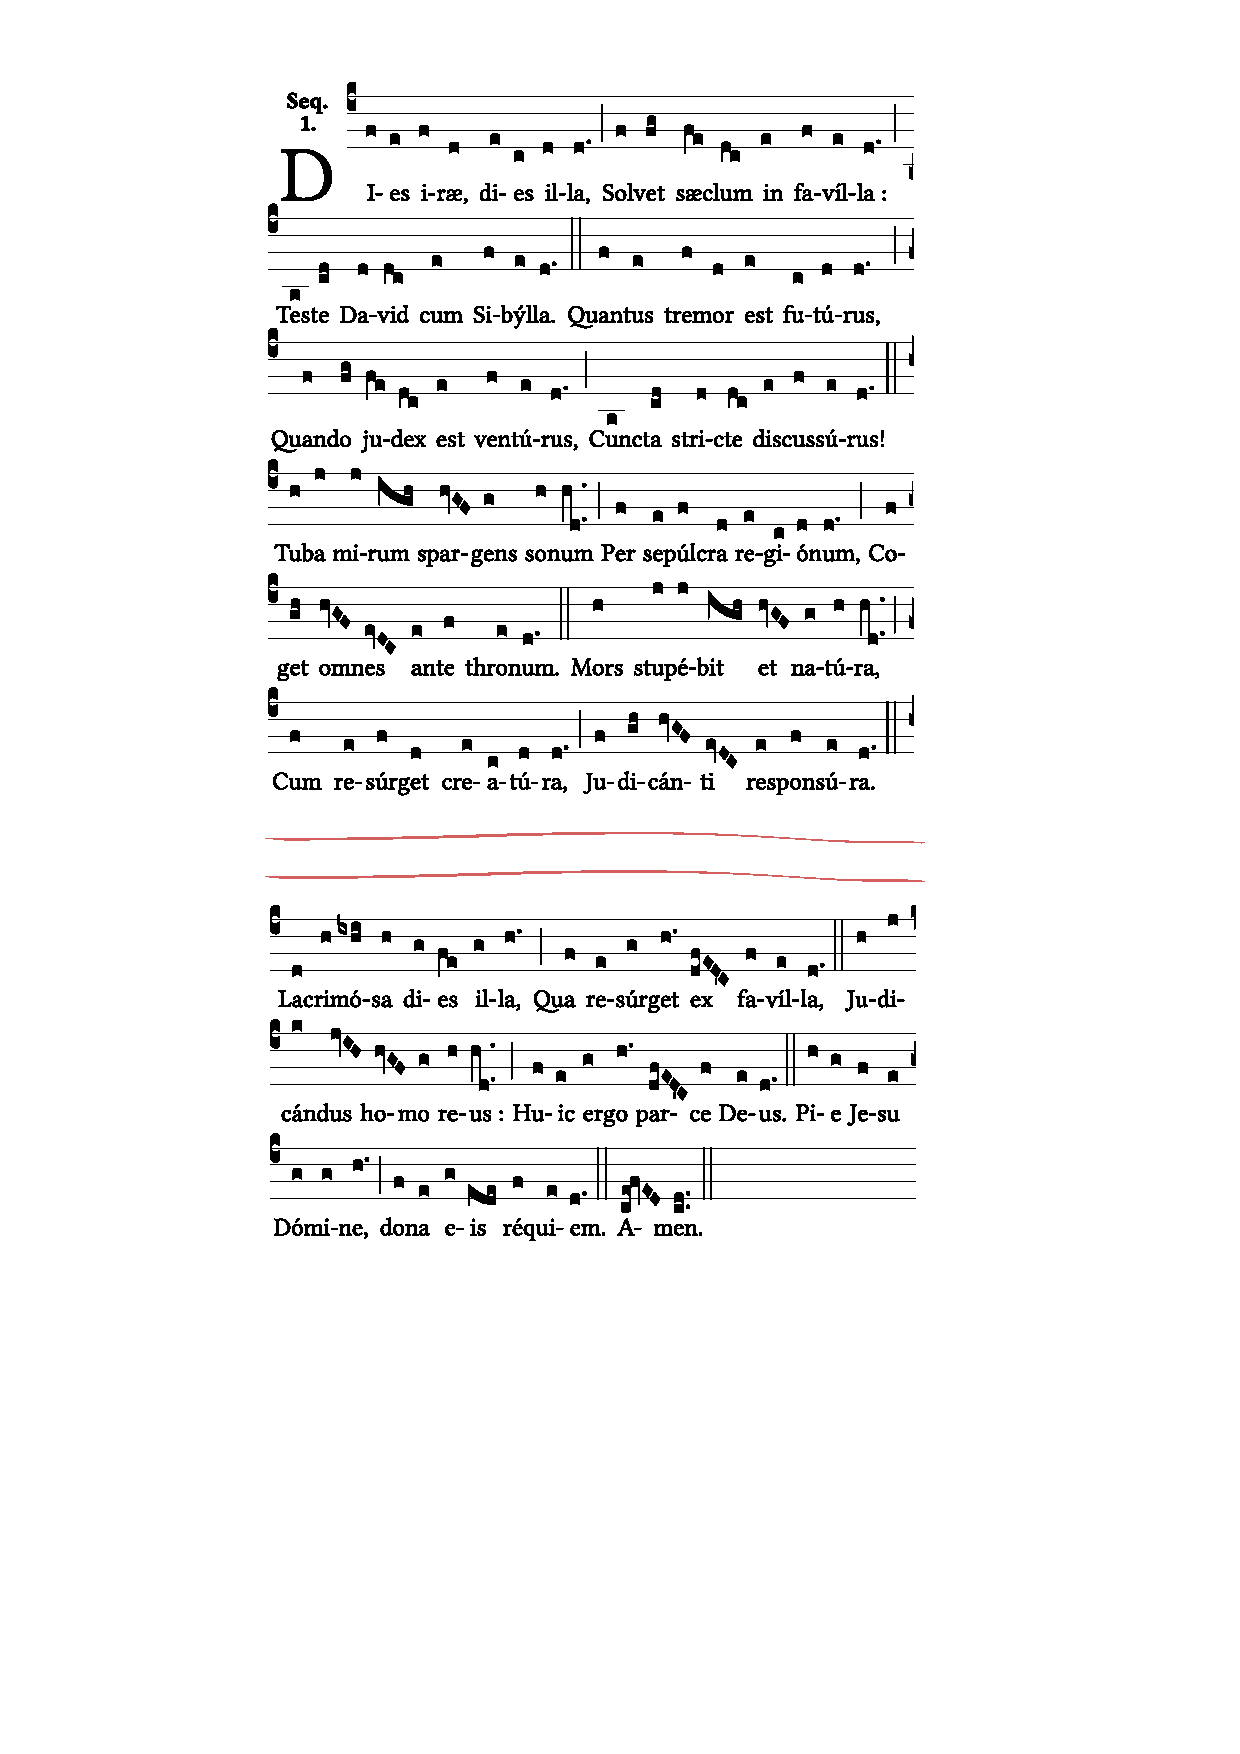
\includegraphics[width=0.90\textwidth]{ud-03/dies-irae-solesmes-cut.pdf}
    \caption{Secc. do inicio e fin do <<Dies irae>>}
    \label{fig:dies-irae}
\end{figure}
% -----------------------
%
\newpage

%\newpage
%
% EXERCICIO 4.- Comentario de textos
% ----------------------------------

\section*{O pensamento musical na Idade
Media}\label{o-pensamento-musical-na-idade-media}

O concepto ---e a expresión--- de «Idade Media» foi creado polos
humanistas europeos do Renacemento para referirse ao período que
separaba a Antigüedad clásica da Modernidade que eles mesmos
representaban. A súa admiración extrema pola arte e o pensamento dos
\emph{antigos} gregos e romanos e o seu desexo de recuperalos nunha
idade \emph{moderna} leváronos ao desprezo por toda a etapa
\emph{intermedia} entre ambos mundos, ignorando ou rexeitando toda
evolución artística, científica e filosófica desa época. Sería moito
máis tarde, xa no século XIX, cando os artistas e pensadores de Europa
rescatarían esa «Idade Media» e farían dela un período mítico de ideais
``caballerescos'', amorosos e relixiosos, nun enfoque igualmente tan
erróneo como o dos seus predecesores.


En realidade, o período que seguimos denominando \emph{medieval} é unha
continuación directa da época clásica, sen presentar unha ruptura clara;
mais nos aproximadamente mil anos que atribuímos a esa época sucedéronse
numerosas formulacións novas en canto á arte ou ao pensamento, e tamén
en canto ao pensamento musical. As ideas e o pensamento musical medieval
foi en gran parte unha prolongación do antigo, onde as ideas principais
quedaron «fosilizadas» durante séculos, houbo tamén enfoques novos desas
mesmas ideas; e, o que é máis importante, formulacións absolutamente
novas, en especial no que respecta á música práctica, tanto nos seus
aspectos técnicos e sistemáticos como na pedagoxía musical; e, de
maneira aínda máis relevante, na escritura musical.

\begin{figure}[h]
\centering
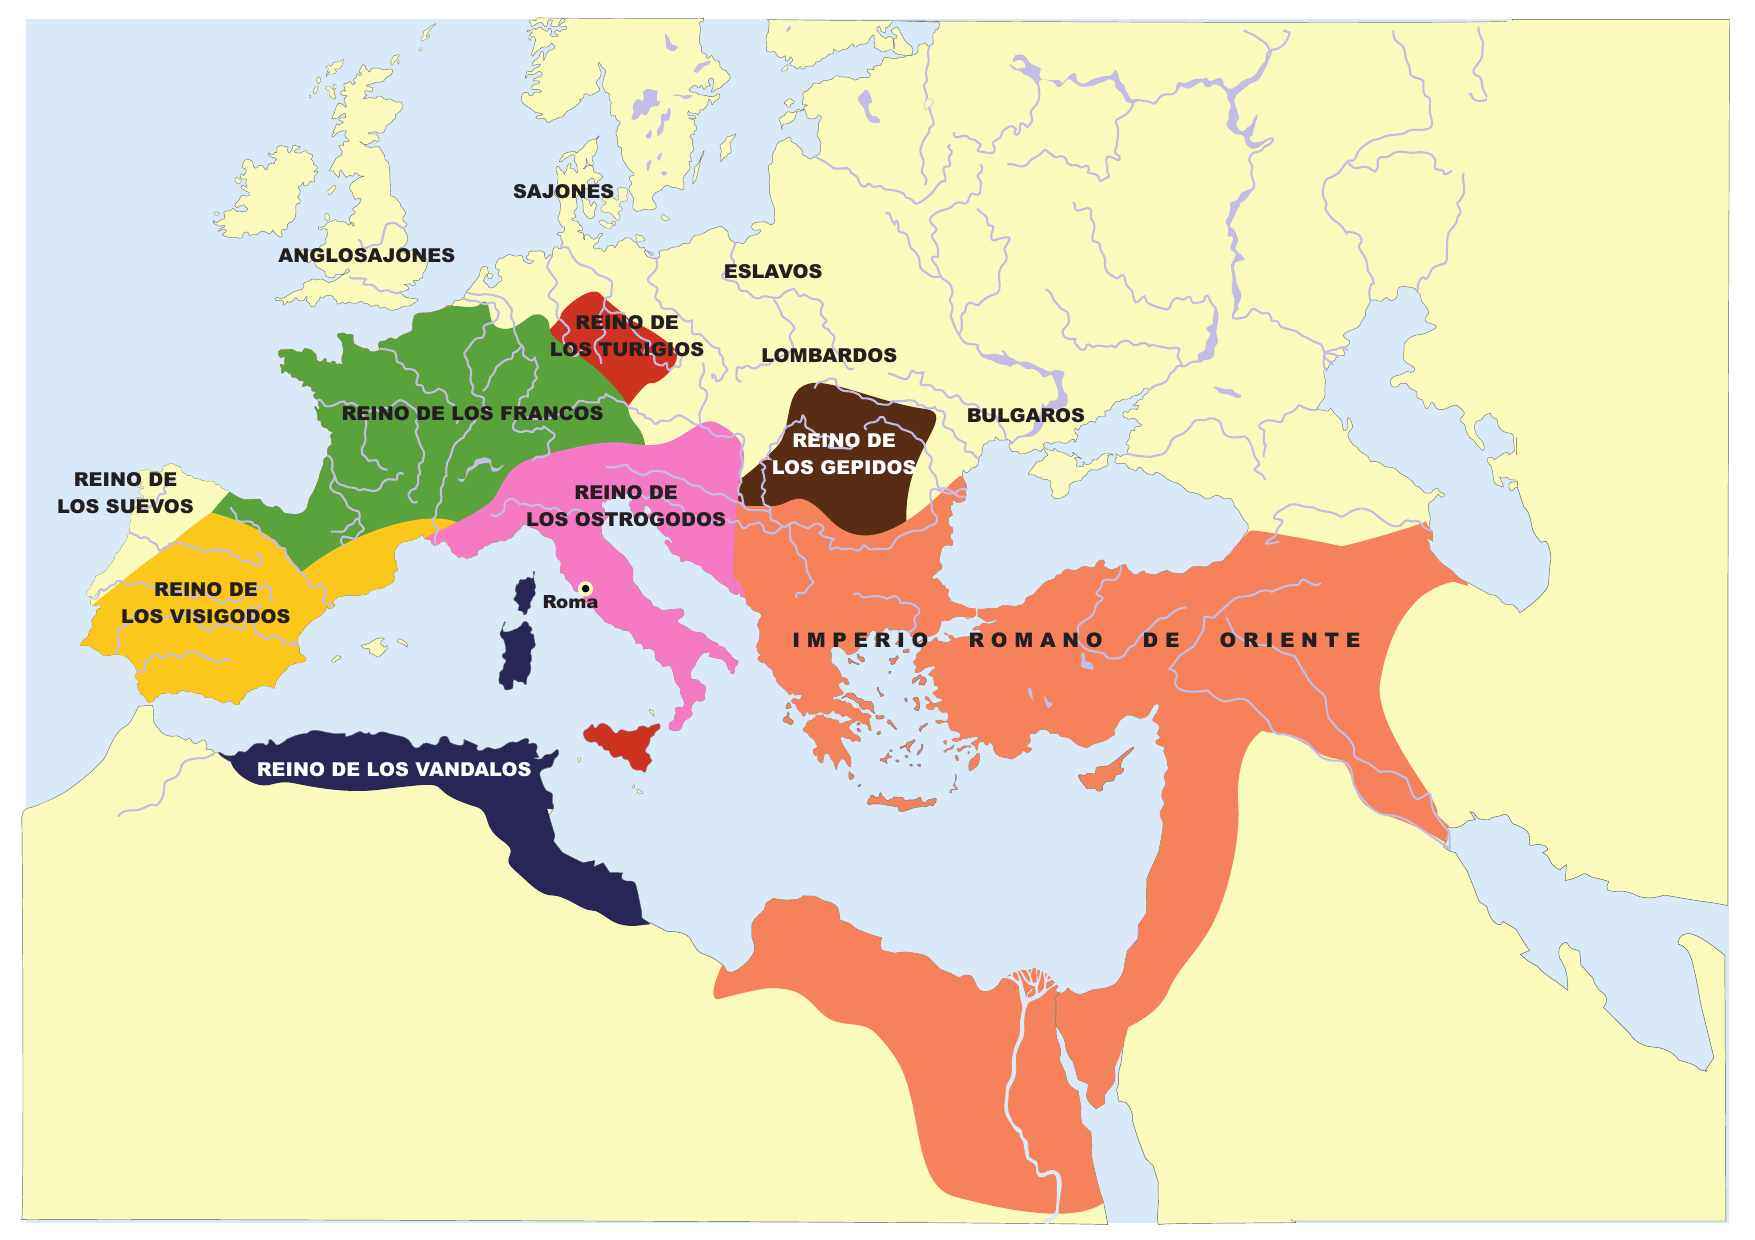
\includegraphics[scale=0.55]{ud-03/mapa_reinos_germanicos.png}
\caption{División política do Mediterráneo c.a 500.\\
(Fonte: Banco de recursos pntic - mec)}
\label{fig:mapa-xermanicos}
\end{figure}

\begin{multicols}{2}

\subsection*{Contexto histórico}\label{o-contexto-historico}

O comezo da Idade Media adoita situarse cara o ano 476 d.C, coincidindo
coa caída do imperio romano de occidente, se ben en realidade isto foi
só a constatación «oficial» de algo que levaba sucedendo desde case dous
séculos antes: a ruptura entre o Oriente \emph{romano} ---que
denominamos \emph{bizantino}--- e o Occidente \emph{xermanizado}, no que
as estruturas do Imperio desapareceran case na súa totalidade.

O período fundamental neste proceso de cambio foi o século IV, en
especial durante os mandatos dos emperadores Constantino, ao comezo do
século, e Teodosio, ao final. Ambos tomaron decisións que influirían
decisivamente no futuro do Imperio: no 313, Constantino decretou o
\emph{Edicto de Milán}, polo que se permitía a liberdade relixiosa e
finalizaban as persecucións; ata entón Roma fora bastante tolerante en
materia relixiosa, pero o culto ao emperador e a certos deuses era
obrigatorio, o cal afectaba principalmente as relixións monoteístas. O
edicto\footnote{As consecuencias do Edicto de Milán foron máis aló do
  recoñecemento da liberdade relixiosa para os cristiáns. Esta
  proclamación conlevou cambios profundos dentro do Imperio romano, así
  como a expansión da Igrexa e o aumento paulatino do seu poder. O
  contido literal do edicto non outorgaba ao cristianismo unha
  importancia especial, xa que se refire á liberdade de cada cidadán de
  practicar a relixión que elixise. O edicto significou a devolución dos
  lugares de culto aos cristiáns, así como das propiedades que foran
  confiscadas polos romanos e vendidas a particulares. Isto deu ao
  cristianismo un maior recoñecemento legal, ata poñerse ao mesmo nivel
  que a relixión romana. Algúns anos máis tarde, converteuse na relixión
  oficial do Imperio e dos seus exércitos. Co Edicto de Milán, o
  paganismo deixou ser a relixión oficial do Imperio romano. A partir
  dese momento, os cristiáns tiveron os mesmos dereitos que o resto dos
  cidadáns.} foi especialmente beneficioso para o cristianismo, que por
entón comezaba a estenderse entre as clases altas do Imperio; a partir
deste edicto, as conversións entre a aristocracia imperial foron
numerosas, converténdose \emph{de feito} na relixión do Imperio; isto
foi ratificado no ano 392 por Teodosio, que proclamou o cristianismo
como relixión \emph{oficial}.

Por outra banda, Constantino mandou edificar unha cidade sobre o
emprazamento da antiga Bizancio, xunto ao Bósforo, para convertela en
capital do Imperio. Isto era a proba definitiva da decadencia da cidade
de Roma, que desde tempo atrás deixara de ser sede imperial. O traslado
da capitalidade á nova Constantinopla supoñía un reforzo da zona
oriental ---grega--- do Imperio, en prexuízo da occidental latina.\\
O deterioro desta última agravouse coa decisión de Teodosio, ao seu
pasamento, de dividir o control do Imperio entre os seus dous fillos:
Arcadio, o maior, gobernaría como emperador desde Constantinopla e
Honorio, sometido ao seu irmán, gobernaría Occidente, primeiro desde
Milán e despois desde Ravena. Esta situación manteríase oficialmente ata
o 476, a pesares de que Occidente experimentaría unha progresiva
\emph{xermanización}, co asentamento de varios pobos (principalmente
visigodos, ostrogodos e francos) que acabaría coa súa fragmentación en
diversos reinos, teoricamente sometidos ao emperador romano de Oriente.
Esta situación complicarase a partir do século VII coa expansión do
Islam despois da morte de Mahoma: o espazo do antigo Imperio Romano
dividirase así en tres zonas diferenciadas no terreo relixioso, político
e cultural: o Imperio, de cultura grega e relixión cristiá ortodoxa; o
mundo árabe musulmán; e o Occidente xermano-latino e católico.

Os primeiros séculos da Idade Media ---coñecidos habitualmente como
«Alta Idade Media»--- caracterízanse en Occidente, ademais de por esta
fragmentación, por unha progresiva \emph{ruralización}, co abandono das
cidades e a desaparición das súas institucións. A nobreza,
principalmente guerreira á maneira xermánica, instálase no medio rural
en castelos e fortalezas illadas. A única institución do Imperio que
permanece forte é a Igrexa, cada vez máis ruralizada tamén, cos
mosteiros como focos importantes. A actividade cultural será exclusiva
destes mosteiros, que aportan unha influencia notable do relixioso sobre
a cultura da época.
Esta situación mantense practicamente ata o século XII, con momentos
relevantes de «renacemento» cultural, como a corte de Carlomagno en
Aquisgrán entre os séculos VIII e IX ou o florecemento do movemento trovadoresco en
\href{https://es.wikipedia.org/wiki/Aquitania}{Aquitania} no século XII.
A partir do século XI, con todo, comeza unha nova etapa, a «Baixa Idade
Media», cunha reurbanización progresiva: as institucións culturais
principais xa non serán só os mosteiros, senón as catedrais e, de modo
moi especial, as universidades, a partir da fundación da Universidade de
Bolonia no 1088; os nobres, especialmente os monarcas, tamén se
instalarán en palacios urbanos. Isto provocará un importante avance
cultural que conducirá en definitiva ao Renacemento.

\subsection*{O pensamento musical}\label{o-pensamento-musical}

\subsubsection*{Alta Idade Media}\label{alta-idade-media}

Durante a Alta Idade Media non se produce unha ruptura importante coas
ideas musicais anteriores, salvo a progresiva «cristianización» das súas
teorías. Mantéñense así a teoría da \emph{harmonía das esferas} (coa
única modificación ---importante--- da intervención divina) e a teoría
do \emph{ethos}, que se relacionará agora cos distintos modos da música
medieval, especialmente a relixiosa. O principal «responsable» desta
continuidade é o filósofo romano \textbf{Severino Boecio}, que crea o
tratado \emph{De institutione musica}, moi citado ---e copiado---
durante toda a Idade Media e moito despois.

A primeira cuestión estritamente medieval, que aparece xa no século IV,
é o debate sobre a conveniencia ou non do uso da música nas cerimonias
relixiosas: a postura dominante é contraria, en principio, dada a
sensualidade da música. Así, en palabras do escritor cristián Lactancio:

\begin{quote}
\small{
O pracer dos oídos orixínase na suavidade das voces e dos cantos; e
inclina ao \emph{vicio} tanto como o dos ollos, como dixemos.}\footnote{Lucio
  Cecilio Firmiano Lactancio (c. 245 -c. 325) foi un escritor latino e
  apoloxista
  cristián do norte de África, discípulo do maestro africano de
  retórica
  \href{https://es.wikipedia.org/wiki/Arnobio_de_Sicca}{Arnobio}.}
\end{quote}

Fronte a esta postura, outros, como
Ambrosio de Milán ou Agustín de Hipona, defenden o uso da música:

\begin{quote}
\small{A quen elevar este canto senón a Deus?}
\end{quote}

Outro debate central durante toda a Idade Media, herdanza tamén do mundo
antigo, é a oposición entre música teórica e música práctica, definida
na época medieval cos termos de músico e \emph{cantor}. O «músico» é o
teórico que coñece os fundamentos da ciencia musical, especialmente a
súa base matemática; o «cantor», pola súa banda, é quen leva á práctica
a música, como un oficio. O prestixio da ciencia e o desprezo polo
traballo manual que caracteriza boa parte do pensamento medieval, fan
que se sitúe tamén por encima o papel do músico fronte ao do cantor; a
música, por outra banda, será parte dos estudos superiores de ciencias,
o \emph{quadrivium}, xunto coa aritmética, a xeometría e a astronomía.

Por último, hai que ter en conta que o sistema de escritura musical que
se utilizou desde o século IV a.C deixa paulatinamente de usarse a
partir do século II d.C, o que leva a desenvolver na Alta Idade Media a
idea de que a música reside só na memoria, e é por tanto un exemplo da
fugacidade. En palabras de
\href{https://es.wikipedia.org/wiki/Isidoro_de_Sevilla}{Isidoro de
Sevilla}:

\begin{quote}
\small{
Se os sons non se reteñen na memoria humana, perecen, xa que non poden
escribirse.
}
\end{quote}

\subsubsection*{Baixa Idade Media}\label{baixa-idade-media}

As teorías indicadas séguense mantendo sen apenas modificación durante
toda a Idade Media, case sempre repetindo literalmente as palabras de
Boecio. Con todo, a partir do século IX comeza unha nova liña nas
formulacións musicais que terá un peso decisivo nos últimos séculos
medievais: trátase da importancia dada á música práctica, tanto nos seus
aspectos máis técnicos (sistema musical) como nos didácticos, entre os
que se incluiría o interese cada vez maior por desenvolver unha notación
musical adecuada.

No primeiro aspecto hai que partir dos tratados anónimos \emph{Musica
enchiriadis} e \emph{Scolica enchiriadis}, ambos do século IX, que xunto
cos libros de \href{https://es.wikipedia.org/wiki/Hucbaldo}{Hucbaldo}
inauguran toda unha serie de tratados musicais que chegará ata o mesmo
Renacemento. En todos estes tratados inclúense habitualmente as teorías
antigas sobre a música, pero a súa formulación central é sempre a
sistematización da música da súa época, clasificada en modos aos que se
adoita atribuír un \emph{ethos} determinado. Tratan tamén aspectos
referentes á interpretación musical, como o uso da ornamentación e da
polifonía improvisada.

Na mesma liña, e cunhas características pedagóxicas importantes, hai que
situar a obra de \textbf{Guido d'Arezzo} (século XI), que desenvolveu un
sistema didáctico baseado en
\href{https://es.wikipedia.org/wiki/Mano_guidoniana}{hexacordos} en que
cada nota estaba asociada a unha sílaba mnemotécnica (a base do actual
solfexo), así como un sistema organizado de notación musical que se
impuxo rapidamente e que evolucionou despois ata o sistema actual.

Por último, o debate sobre a conveniencia da música que se orixinou no
século IV, continuará na Baixa Idade Media asociado agora á polifonía e
os seus diferentes estilos, considerados en ocasións como inadecuados
para o seu uso litúrxico.

\end{multicols}

\begin{ejercicio}[Pensamento musical Idade Media]
\begin{enumerate}[1.-]
 \item
 Resume brevemente as características do pensamento musical na Alta Idade Media.
 \vspace*{6.60cm}
 \item
 Indica de xeito resumido as características do pensar musical na Baixa Idade Media.
 \vspace*{6.6cm}
\end{enumerate}


% ESPACIO PARA REDACTAR O COMENTARIO DA AUDICIÓN
%
%\small{}
%\small{Trátase dunha forma vocal menor, de estrutura ternaria; segundo o ámbito e estilo, obedece a un canto antifonal do propio da misa cantado a capella por un coro de voces masculinas; a textura monódica horizontal é propia do canto chá (Gregoriano) en estilo neumático na primeira sección e silábico na segunda, de ámbito reducido escrita no modo \textit{tetrardus auténtico} (VII)     }

\end{ejercicio}
%\begin{figure}[h!]
%\centering
%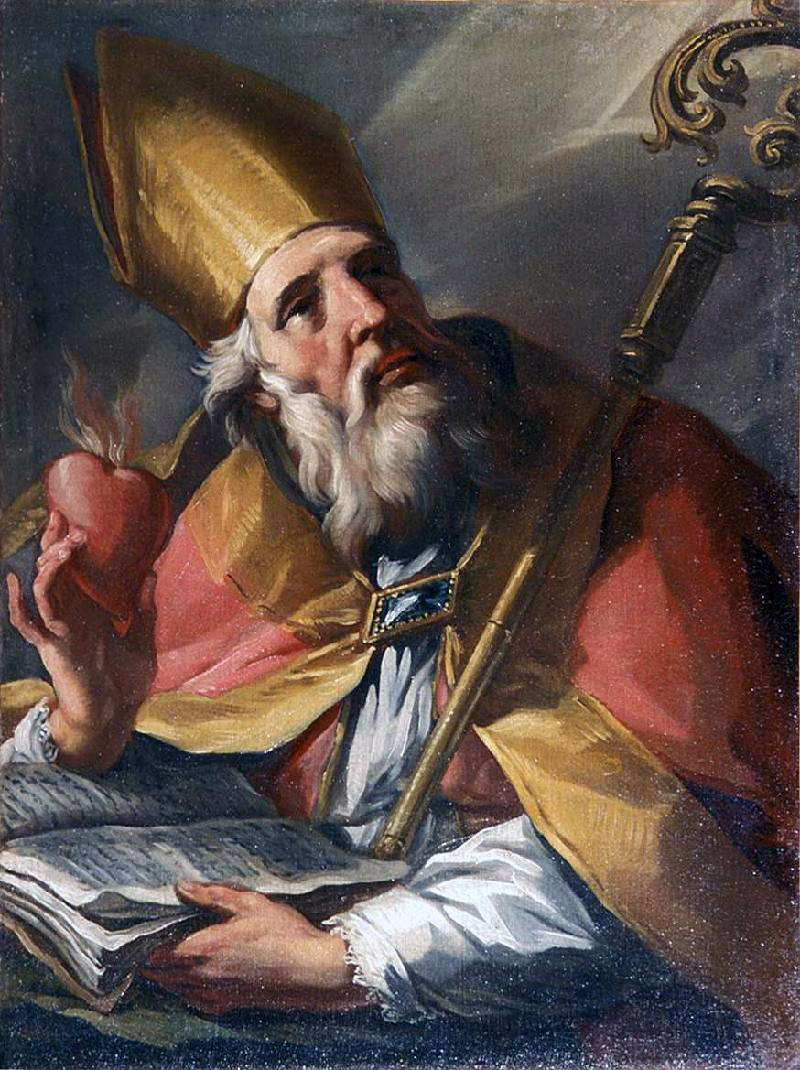
\includegraphics[width=0.5\textwidth]{ud-03/SanAgustin.jpg}
%\caption{San Agustín canonizado.\\
%(Fonte: wikimedia commons)}
%\label{fig:San-Agustin}
%\end{figure}


%
% TEXTOS SOBRE O PENSAMENTO MUSICAL
% ---------------------------------
% Agustín de Hipona (San Agustín)
%
\begin{multicols}{2}
%
\subsection*{Pensadores e textos}\label{pensadores-textos}
%
\paragraph{\texorpdfstring{Agustín de Hipona (354-430), \emph{Comentarios
aos salmos}}{Agustín de Hipona (354-430), Comentarios aos salmos}}\label{agustuxedn-de-hipona-354-430--comentarios-aos-salmos}
%
%
Agustín de Hipona é un dos denominados «Pais da Igrexa», é dicir, os primeiros pensadores que desenvolveron nos seus escritos a filosofía do cristianismo. Naceu en Tagaste ( Alxeria) e estudou en Cartago. Inicialmente pagán, converteuse ao cristianismo durante a súa estancia en Milán, onde coñeceu ao bispo Ambrosio; el mesmo chegou a ser bispo de Hipona (Alxeria). Foi canonizado pola igrexa católica. 
Nos seus numerosos escritos hai constantes referencias á música; mesmo escribiu un tratado completo, \emph{De musica}, do que só se conserva unha parte. O seguinte texto, defende e aconsella o uso da música nos cantos relixiosos, fronte á opinión xeral dos bispos da súa época.
%
%\begin{figure}[h]
%\centering
%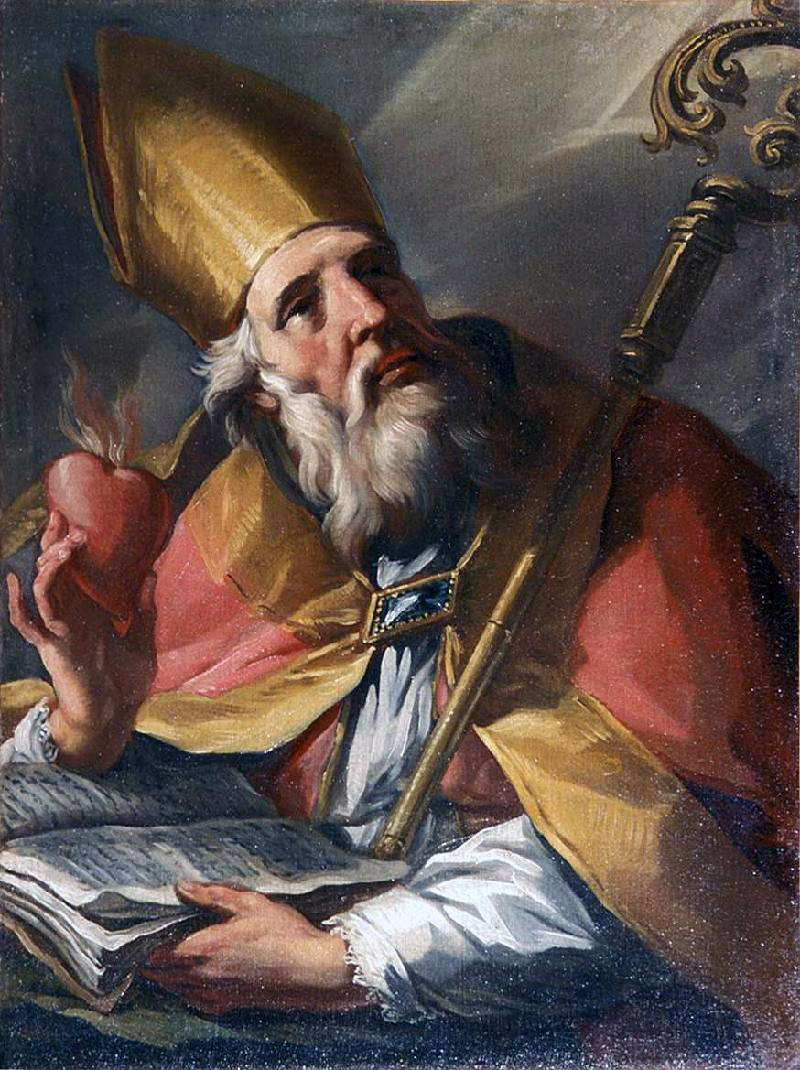
\includegraphics[width=0.5\textwidth]{ud-03/SanAgustin.jpg}
%\caption{San Agustín canonizado.\\
%(Fonte: wikimedia commons)}
%\label{fig:San-Agustin}
%\end{figure}
%
\begin{Figura}
  \centering
  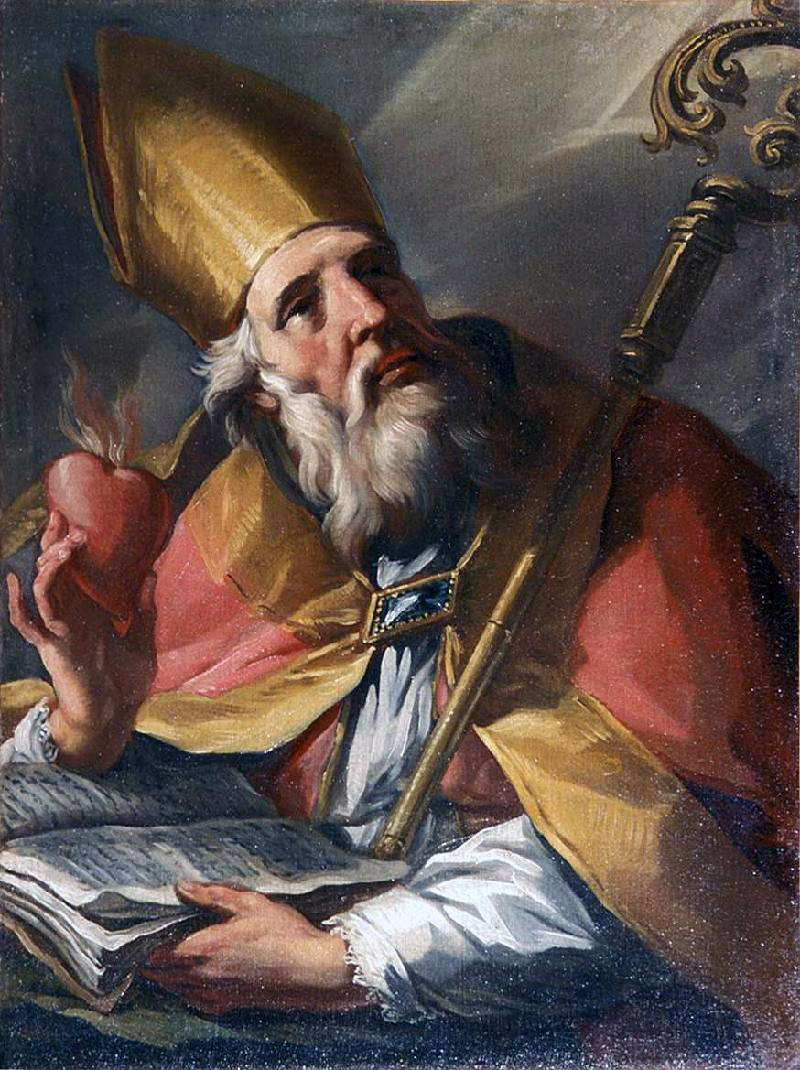
\includegraphics[width=0.75\textwidth]{ud-03/SanAgustin.jpg}
  \captionof{figure}{San Agustín canonizado.\\
  (Fonte: wikimedia commons)}
  \label{fig:San-Agustin}
\end{Figura}
%
\end{multicols}
%
\begin{quote}
\small{
``Velaquí que El case che dá o ton da melodía a cantar: non vaias en busca
do texto, coma se puideses traducir en sons articulados un canto no que
Deus se recree. Canta no xúbilo. Cantar con arte a Deus consiste niso:
cantar no xúbilo. Que significa cantar no xúbilo? Comprender e non saber
explicar en palabras o que se canta co corazón. Aqueles que cantan
durante a sega, ou durante a vendima, ou durante calquera outro
traballo, primeiro advirten o pracer que suscita o texto dos cantos,
pero máis tarde, cando a emoción crece, senten que non poden expresala
en palabras e entón desafóganse nunha soa modulación de notas. Este
canto denominámolo xúbilo.\\
O xúbilo é esa melodía coa que o corazón expresa todo o que non pode
expresar con palabras. E a quen elevar este canto senón a Deus? En
efecto, El é o que ti non podes expresar. E se non o podes expresar e
tampouco calalo, que outra cousa podes facer máis que xubilar? Entón o
corazón abrirase á alegría, sen utilizar palabras, e a grandeza
extraordinaria da alegría non coñecerá os límites das sílabas.
Cantádelle con arte no xúbilo.''
}
\end{quote}
%
\begin{ejercicio}[Pensamento musical Idade Media]
  \begin{enumerate}[1.-]
  \item
    En que época das que coñeces da Idade Media desenvolve as súas ideas sobre a música San Agustín? \ldots
%    \vspace*{0.5cm}
  \item
    Sinala no texto as palabras que fan referencia á concepción sobre música de San Agustín. \\
    Que cres que é para o autor ``cantar con xúbilo''? Consideras que está 
a favor ou en contra do uso do canto na Igrexa? Xustifica a túa resposta.
    \vspace*{3.10cm}
  \end{enumerate}
\end{ejercicio}

%\newpage
%
% EXERCICIO 5.- Cuestións de repaso
% ---------------------------------
%
% TEXTOS SOBRE O PENSAMENTO MUSICAL
% ---------------------------------
% Agustín de Hipona (San Agustín)
%
\begin{multicols}{2}
%
%\subsection*{Pensadores e textos}\label{pensadores-textos}
%
\paragraph{Boecio (470-524): \emph{Tratado de música}}\label{Boecio-tratado}
%
Severino Boecio, o máis relevante teórico musical no tránsito á Idade Media, foi un alto funcionario da corte ostrogoda, que terminou condenado á morte polo rei Teodorico. No cárcere escribiu a súa obra máis famosa, \emph{El consuelo de la filosofía}.\\
Boecio proxectou realizar un gran compendio das ciencias da súa época, chamadas entón artes liberais; a pesar de que non se concluíu, si redactou algúns tratados, entre eles o referido á música. Este tratado converteuse en libro de referencia de todos os teóricos musicais durante a Idade media e tamén no Renacemento, e os seus contidos foron repetidos case literalmente durante séculos.

No comezo do tratado, Boecio realiza unha clasificación das partes da música que se faría tópica posteriormente. Este é o texto que segue.
%
%\begin{figure}[h]
%\centering
%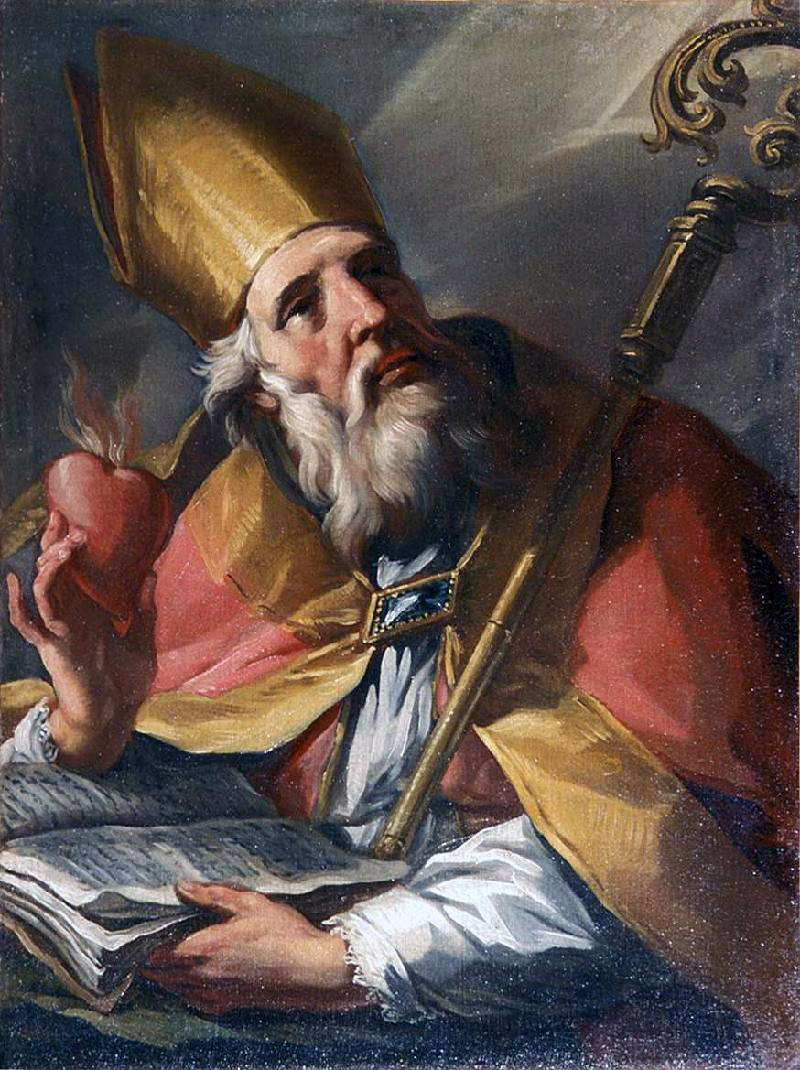
\includegraphics[width=0.5\textwidth]{ud-03/SanAgustin.jpg}
%\caption{San Agustín canonizado.\\
%(Fonte: wikimedia commons)}
%\label{fig:San-Agustin}
%\end{figure}
%
\begin{Figura}
  \centering
  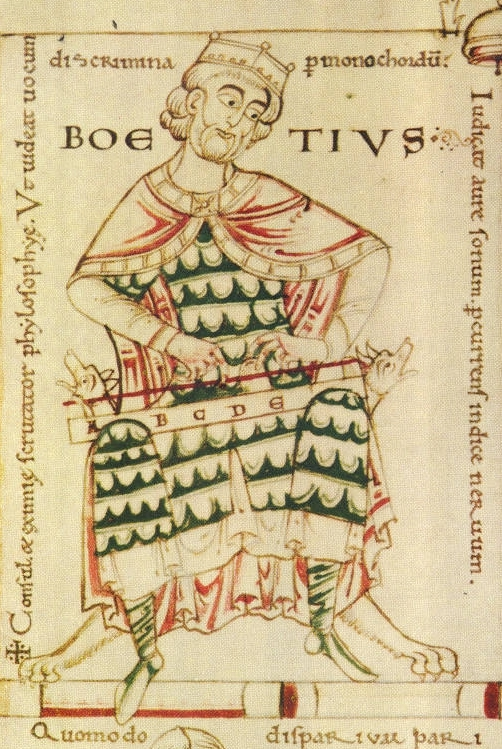
\includegraphics[width=0.75\textwidth]{ud-03/boecio.jpg}
  \captionof{figure}{Severino Boecio (470-524).\\
  (Fonte: wikimedia commons)}
  \label{fig:Severino-Boecio}
\end{Figura}
%
\end{multicols}
%
\vspace*{0.05cm}
\begin{quote}
\small{
``Aquel que escribe de música debe saber exponer en primer lugar las partes en que los estudiosos han subdividido la materia. Estas son tres: la primera está formada por la música del universo (mundana); la segunda por la música humana, y la tercera por la música instrumental, como la de la cítara, de las flautas y de los demás instrumentos con los que se puede obtener una melodía.

La música del universo, que hay que estudiar sobre todo en los cielos, es resultado de la unión de los elementos o de la variación de las estaciones. ¿Cómo podría moverse en carrera muda y silenciosa el mecanismo del cielo tan veloz? A pesar de que tal sonido no llegue a nuestro oído —y ello sucede necesariamente por múltiples razones— el movimiento rapidísimo de cuerpos tan enormes no puede darse sin sonido alguno, especialmente porque los movimientos orbitales de los astros están vinculados en una relación tan perfecta que no se puede imaginar nada más compacto y proporcionado. En efecto, algunos se mueven más arriba y otros más abajo, girando todos ellos con un impulso tan bien combinado que sus diferentes velocidades dan lugar a un orden racional en los movimientos. Por ello no puede ser ajeno a este movimiento rotatorio de los cielos el orden racional en la modulación de los sonidos. [...]

Todos pueden comprender lo que significa la música humana examinándose a sí mismos. En efecto, ¿qué une al cuerpo la incorpórea vitalidad de la mente sino una relación ordenada, como si se tratase de una justa combinación de sonidos graves y agudos para producir una única consonancia? Además, ¿qué podría asociar entre sí las partes del alma, la cual —según la doctrina de Aristóteles— es resultado de la fusión de lo irracional con lo racional? Y también: ¿qué podría mezclar los elementos del cuerpo y combinar sus partes con una relación ordenada? Pero de esto también trataremos más adelante.

La tercera parte de la música es la que se considera propia de algunos instrumentos. Es producida por la tensión, como en la cuerda; por el aire, como en las flautas, o en otros instrumentos activados por el agua; por la percusión, como en los instrumentos cuya concavidad es golpeada con una maza de bronce, dando lugar a sonidos diversos.''
}
\end{quote}
%
\begin{ejercicio}[Pensamento musical Idade Media]
  \begin{enumerate}[1.-]
  \item
    En que época das que coñeces da Idade Media desenvolve no seu tratado as ideas sobre a música Boecio? \ldots
%    \vspace*{0.5cm}
  \item
    Sinala no texto aquelas palabras que destacarías sobre a concepción da música de Boecio. \\
    Que cres que é para o autor ``cantar con xúbilo''? Consideras que está a favor ou en contra do uso do canto na Igrexa? Xustifica a túa resposta.
    \vspace*{3.10cm}
  \end{enumerate}
\end{ejercicio}

%\newpage
%
% EXERCICIO 6.- Comentario «A Chantar»
% ------------------------------------
%
% TEXTOS SOBRE O PENSAMENTO MUSICAL
% ---------------------------------
% Agustín de Hipona (San Agustín)
%
\begin{multicols}{2}
%
%\subsection*{Pensadores e textos}\label{pensadores-textos}
%
  \paragraph{Hildegard de Bingen (1098-1179): \emph{Epístola a los prelados de Magnucia}}\label{Hildegard de Bingen}
%
  Hildegard de Bingen é un dos personaxes máis da Idade media. Foi abadesa do convento de Rupertsberg, que ela mesma fundara. As súas dedicacións foron moi diversas: era experta en botánica, medicina e outras ciencias; escribiu numerosos libros de visións proféticas que lle valeron o sobrenome de ``Sibila do Rin''; foi conselleira de papas, bispos, emperadores e reis; compuxo numerosas pezas musicais e obras teatrais con música. No seu amplo epistolario, dirixido a numerosas personalidades da súa época, trata moi diversos temas.

  A \emph{epístola aos prelados de Maguncia} xorde dunha situación concreta: este bispado, ao que pertencía o convento de Rupertsberg, prohibira á comunidade cantar o oficio, tras un conflito polo enterro en sagrado dun excomungado. A abadesa responde facendo unha contundente defensa da música.

\begin{Figura}
  \centering
  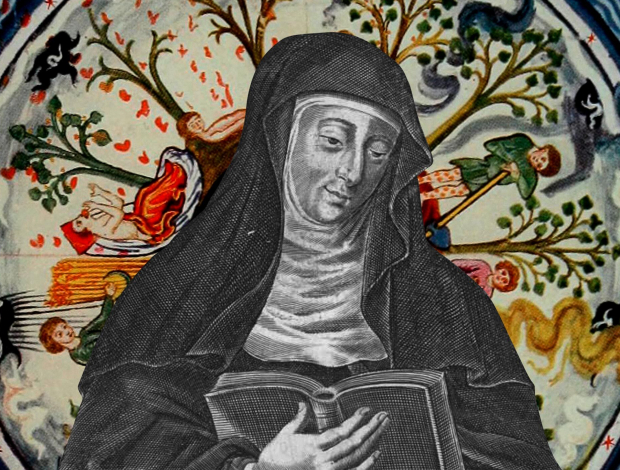
\includegraphics[width=0.75\textwidth]{ud-03/Hildegard de Bingen.jpg}
  \captionof{figure}{Hildegard de Bingen (1098-1179).\\
  (Fonte: wikimedia commons)}
  \label{fig:Hildegard-Bingen}
\end{Figura}
%
\end{multicols}
%
\vspace*{0.05cm}
\begin{quote}
\small{
Y vi algo más —pues en obediencia vuestra hemos dejado de cantar el Divino Oficio, celebrándolo solo con la lectura en silencio— y oí una voz que venía de la luz viva, hablando de las diversas formas de alabanza de las que habla David en los Salmos: «Alabadlo con el sonido de la trompeta, alabadlo con el salterio y la cítara, alabadlo con el tímpano y el coro, alabadlo con las cuerdas y el órgano, alabadlo con los sonoros címbalos, alabadlo con los címbalos del júbilo. Que todo espíritu alabe al Señor». [...] Cuando nos esforzamos seriamente en alabarlo, rememoramos cómo buscó el hombre la voz del Espíritu vivo, que Adán perdió por su desobediencia [...] Pues Adán perdió esa semejanza con la voz angélica que tuvo en el Paraíso, y así se durmió esa ciencia musical de que estaba dotado antes de su pecado. Pero Dios, que repone las almas de los elegidos en su estado original de felicidad por la luz de la verdad, forjó en su sabiduría esto: que cuando el Espíritu, con una infusión profética, renovara el corazón de muchos, recobraran estos por esta iluminación interior todo lo perdido de lo que poseía Adán antes del castigo.

Y para que la humanidad, más que rememorar el destierro de Adán, fuera despertada también a estas cosas —la divina dulzura y la alabanza que había disfrutado Adán antes de su caída—, los mismos profetas, enseñados por el Espíritu que habían recibido, no solo compusieron salmos y cánticos, que se cantarían para encender la devoción de quienes los oyeran, sino que también inventaron diversos instrumentos del arte musical, que serían tocados con gran variedad de sonidos. Lo hicieron para que los oyentes, tanto por el sonido de estos instrumentos como por el sentido de las palabras cantadas con su acompañamiento, fuesen educados en asuntos del interior, impulsados y espoleados por objetos exteriores. Hombres sabios y aplicados imitaron a estos santos profetas e inventaron numerosos tipos de instrumentos humanos, de modo que pudieran hacer música para el deleite de sus almas y adaptar lo que cantaban con las pulsaciones de sus dedos, como rememorando que Adán fue formado por el dedo de Dios (que es el Espíritu Santo); ese Adán en cuya voz, antes de su caída, residía el sonido de toda armonía y la dulzura de todo el arte musical; y si hubiera permanecido en el estado en que fue creado, la fragilidad de los hombres mortales no podrían soportar la potencia y sonoridad de su voz. [...]

Por tanto, quienes sin una razón segura y de peso imponen silencio en la iglesia en materia de cantos de alabanza a Dios, y privan así injustamente a Dios de su alabanza en la tierra, serán asimismo privados de la participación en las alabanzas angélicas que se oyen en el Cielo, salvo que hagan reparación por arrepentimiento sincero y penitencia humilde.
}
\end{quote}
%
\begin{ejercicio}[Pensamento musical Idade Media]
  \begin{enumerate}[1.-]
  \item
    En que época das que coñeces da Idade Media sitúas cronolóxicamente a autora do anterior texto? \ldots
%    \vspace*{0.5cm}
  \item
    Sinala no texto aquelas palabras que destacarías sobre a concepción da música da autora. \\
    \vspace*{8.10cm}
  \end{enumerate}
\end{ejercicio}

%\newpage
%
% EXERCICIO 7.- 
% -------------
%%
% ----
\hideanswers % oculta respostas
%
% Cargamos os Exercicios:
% ----------------------

\loadallproblems[Tema3-GREGO]{../../Cuestions/Tema3-Canto-gregoriano.tex}

\loadallproblems[Tema3-GREGO1]{../../Cuestions/Tema3-Canto-gregoriano-expansion.tex} %
%\loadallproblems[Tema3-NOTA]{../../Cuestions/Tema3-Notacion-modal.tex} %
%\loadallproblems[Tema1-PENS]{../../Cuestions/Tema1-Pensamento.tex} %
%\loadallproblems[Tema1-RO]{../../Cuestions/Tema1-Roma.tex} %
%\loadrandomproblems[loops]{2}{loops}% aleatorios
%
% FOLLA EXERCICIOS: 
% -----------------
\begin{multicols}{2} % a 2 columnas
    \begin{enumerate}
%\useproblem{input}
    \foreachproblem[Tema3-GREGO]{\item\label{prob:\thisproblemlabel}\thisproblem}
    \foreachproblem[Tema3-GREGO1]{\item\label{prob:\thisproblemlabel}\thisproblem}
 %   \foreachproblem[Tema3-NOTA]{\item\label{prob:\thisproblemlabel}\thisproblem}
%    \foreachproblem[Tema1-PENS]{\item\label{prob:\thisproblemlabel}\thisproblem}
    \end{enumerate}
\end{multicols}
%
% SOLUCIONS:
% ----------
%\newpage
%\begin{multicols}{2}
%\showanswers
%\begin{itemize}
%\foreachdataset{\thisdataset}{%
%\foreachproblem[\thisdataset]{\item[\ref{prob:\thisproblemlabel}]\thisproblem}
%}
%\end{itemize}
%\end{multicols}
%\newpage
%
% EXERCICIO 8.- 
% -------------
%\input{Exercicio-A-Chantar-comentario.tex}
%\newpage
%
% EXERCICIO 9.- 
% -------------
%\input{Exercicio-A-Chantar-comentario.tex}
%\newpage
%
% EXERCICIO 10.- 
% -------------
%\input{Exercicio-A-Chantar-comentario.tex}
%\newpage
%
% EXERCICIO 10.- 
% -------------
%\input{Exercicio-A-Chantar-comentario.tex}
%\newpage
\end{document}
%Fin de Hoja de ejercicios
%
